%-----------------------------------------------------------------------------------------------------------------------------------------------%
%	The MIT License (MIT)
%
%	Copyright (c) 2019 Jan Küster
%
%	Permission is hereby granted, free of charge, to any person obtaining a copy
%	of this software and associated documentation files (the "Software"), to deal
%	in the Software without restriction, including without limitation the rights
%	to use, copy, modify, merge, publish, distribute, sublicense, and/or sell
%	copies of the Software, and to permit persons to whom the Software is
%	furnished to do so, subject to the following conditions:
%
%	THE SOFTWARE IS PROVIDED "AS IS", WITHOUT WARRANTY OF ANY KIND, EXPRESS OR
%	IMPLIED, INCLUDING BUT NOT LIMITED TO THE WARRANTIES OF MERCHANTABILITY,
%	FITNESS FOR A PARTICULAR PURPOSE AND NONINFRINGEMENT. IN NO EVENT SHALL THE
%	AUTHORS OR COPYRIGHT HOLDERS BE LIABLE FOR ANY CLAIM, DAMAGES OR OTHER
%	LIABILITY, WHETHER IN AN ACTION OF CONTRACT, TORT OR OTHERWISE, ARISING FROM,
%	OUT OF OR IN CONNECTION WITH THE SOFTWARE OR THE USE OR OTHER DEALINGS IN
%	THE SOFTWARE.
%
%
%-----------------------------------------------------------------------------------------------------------------------------------------------%


%============================================================================%
%
%	DOCUMENT DEFINITION
%
%============================================================================%

%we use article class because we want to fully customize the page and don't use a cv template
\documentclass[10pt,A4]{article}


%----------------------------------------------------------------------------------------
%	ENCODING
%----------------------------------------------------------------------------------------

% we use utf8 since we want to build from any machine
\usepackage[utf8]{inputenc}

%----------------------------------------------------------------------------------------
%	LOGIC
%----------------------------------------------------------------------------------------

% provides \isempty test
\usepackage{xstring, xifthen}

%----------------------------------------------------------------------------------------
%	FONT BASICS
%----------------------------------------------------------------------------------------

% some tex-live fonts - choose your own

%\usepackage[defaultsans]{droidsans}
%\usepackage[default]{comfortaa}
%\usepackage{cmbright}
\usepackage[default]{raleway}
%\usepackage{fetamont}
%\usepackage[default]{gillius}
%\usepackage[light,math]{iwona}
%\usepackage[thin]{roboto}

% set font default
\renewcommand*\familydefault{\sfdefault}
\usepackage[T1]{fontenc}

% more font size definitions
\usepackage{moresize}

%----------------------------------------------------------------------------------------
%	FONT AWESOME ICONS
%----------------------------------------------------------------------------------------

% include the fontawesome icon set
\usepackage{fontawesome}

% use to vertically center content
% credits to: http://tex.stackexchange.com/questions/7219/how-to-vertically-center-two-images-next-to-each-other
\newcommand{\vcenteredinclude}[1]{\begingroup
\setbox0=\hbox{\includegraphics{#1}}%
\parbox{\wd0}{\box0}\endgroup}

% use to vertically center content
% credits to: http://tex.stackexchange.com/questions/7219/how-to-vertically-center-two-images-next-to-each-other
\newcommand*{\vcenteredhbox}[1]{\begingroup
\setbox0=\hbox{#1}\parbox{\wd0}{\box0}\endgroup}

% icon shortcut
\newcommand{\icon}[3] {
    \makebox(#2, #2){\textcolor{maincol}{\csname fa#1\endcsname}}
}

% icon with text shortcut
\newcommand{\icontext}[4]{
    \vcenteredhbox{\icon{#1}{#2}{#3}}  \hspace{2pt}  \parbox{0.9\mpwidth}{\textcolor{#4}{#3}}
}

% icon with website url
\newcommand{\iconhref}[5]{
    \vcenteredhbox{\icon{#1}{#2}{#5}}  \hspace{2pt} \href{#4}{\textcolor{#5}{#3}}
}

% icon with email link
\newcommand{\iconemail}[5]{
    \vcenteredhbox{\icon{#1}{#2}{#5}}  \hspace{2pt} \href{mailto:#4}{\textcolor{#5}{#3}}
}

%----------------------------------------------------------------------------------------
%	PAGE LAYOUT  DEFINITIONS
%----------------------------------------------------------------------------------------

% page outer frames (debug-only)
% \usepackage{showframe}

% we use paracol to display breakable two columns
\usepackage{paracol}

% define page styles using geometry
\usepackage[a4paper]{geometry}

% remove all possible margins
\geometry{top=1cm, bottom=1cm, left=1cm, right=1cm}

\usepackage{fancyhdr}
\pagestyle{empty}

% space between header and content
% \setlength{\headheight}{0pt}

% indentation is zero
\setlength{\parindent}{0mm}

%----------------------------------------------------------------------------------------
%	TABLE /ARRAY DEFINITIONS
%----------------------------------------------------------------------------------------

% extended aligning of tabular cells
\usepackage{array}

% custom column right-align with fixed width
% use like p{size} but via x{size}
\newcolumntype{x}[1]{%
        >{\raggedleft\hspace{0pt}}p{#1}}%


%----------------------------------------------------------------------------------------
%	GRAPHICS DEFINITIONS
%----------------------------------------------------------------------------------------

%for header image
\usepackage{graphicx}

% use this for floating figures
% \usepackage{wrapfig}
% \usepackage{float}
% \floatstyle{boxed}
% \restylefloat{figure}

%for drawing graphics
\usepackage{tikz}
\usetikzlibrary{shapes, backgrounds,mindmap, trees}

%----------------------------------------------------------------------------------------
%	Color DEFINITIONS
%----------------------------------------------------------------------------------------
\usepackage{transparent}
\usepackage{color}

% primary color
\definecolor{maincol}{RGB}{ 225, 0, 0 }

% accent color, secondary
% \definecolor{accentcol}{RGB}{ 250, 150, 10 }

% dark color
\definecolor{darkcol}{RGB}{ 70, 70, 70 }

% light color
\definecolor{lightcol}{RGB}{245,245,245}


% Package for links, must be the last package used
\usepackage[hidelinks]{hyperref}

% returns minipage width minus two times \fboxsep
% to keep padding included in width calculations
% can also be used for other boxes / environments
\newcommand{\mpwidth}{\linewidth-\fboxsep-\fboxsep}



%============================================================================%
%
%	CV COMMANDS
%
%============================================================================%

%----------------------------------------------------------------------------------------
%	 CV LIST
%----------------------------------------------------------------------------------------

% renders a standard latex list but abstracts away the environment definition (begin/end)
\newcommand{\cvlist}[1] {
    \begin{itemize}{#1}\end{itemize}
}

%----------------------------------------------------------------------------------------
%	 CV TEXT
%----------------------------------------------------------------------------------------

% base class to wrap any text based stuff here. Renders like a paragraph.
% Allows complex commands to be passed, too.
% param 1: *any
\newcommand{\cvtext}[1] {
    \begin{tabular*}{1\mpwidth}{p{0.98\mpwidth}}
        \parbox{1\mpwidth}{#1}
    \end{tabular*}
}

%----------------------------------------------------------------------------------------
%	CV SECTION
%----------------------------------------------------------------------------------------

% Renders a a CV section headline with a nice underline in main color.
% param 1: section title
\newcommand{\cvsection}[1] {
    \vspace{14pt}
    \cvtext{
        \textbf{\LARGE{\textcolor{darkcol}{\uppercase{#1}}}}\\[-4pt]
        \textcolor{maincol}{ \rule{0.1\textwidth}{2pt} } \\
    }
}

%----------------------------------------------------------------------------------------
%	META SKILL
%----------------------------------------------------------------------------------------

% Renders a progress-bar to indicate a certain skill in percent.
% param 1: name of the skill / tech / etc.
% param 2: level (for example in years)
% param 3: percent, values range from 0 to 1
\newcommand{\cvskill}[3] {
    \begin{tabular*}{1\mpwidth}{p{0.72\mpwidth}  r}
        \textcolor{black}{\textbf{#1}} & \textcolor{maincol}{#2}\\
    \end{tabular*}%

    \hspace{4pt}
    \begin{tikzpicture}[scale=1,rounded corners=2pt,very thin]
        \fill [lightcol] (0,0) rectangle (1\mpwidth, 0.15);
        \fill [maincol] (0,0) rectangle (#3\mpwidth, 0.15);
    \end{tikzpicture}%
}


%----------------------------------------------------------------------------------------
%	 CV EVENT
%----------------------------------------------------------------------------------------

% Renders a table and a paragraph (cvtext) wrapped in a parbox (to ensure minimum content
% is glued together when a pagebreak appears).
% Additional Information can be passed in text or list form (or other environments).
% the work you did
% param 1: time-frame i.e. Sep 14 - Jan 15 etc.
% param 2:	 event name (job position etc.)
% param 3: Customer, Employer, Industry
% param 4: Short description
% param 5: work done (optional)
% param 6: technologies include (optional)
% param 7: achievements (optional)
\newcommand{\cvevent}[7] {

% we wrap this part in a parbox, so title and description are not separated on a pagebreak
% if you need more control on page breaks, remove the parbox
    \parbox{\mpwidth}{
        \begin{tabular*}{1\mpwidth}{p{0.72\mpwidth}  r}
            \textcolor{black}{\textbf{#2}} & \colorbox{maincol}{\makebox[0.25\mpwidth]{\textcolor{white}{#1}}} \\
            \textcolor{maincol}{\textbf{#3}} & \\
        \end{tabular*}\\[8pt]

        \ifthenelse{\isempty{#4}}{}{
            \cvtext{#4}\\
        }
    }

    \ifthenelse{\isempty{#5}}{}{
        \vspace{5pt}
        {#5}
    }

    \ifthenelse{\isempty{#6}}{}{
        \vspace{6pt}
        \cvtext{\small\textbf{Skills}}\\
        {#6}
    }
    \vspace{14pt}
}

%----------------------------------------------------------------------------------------
%	 CV META EVENT
%----------------------------------------------------------------------------------------

% Renders a CV event on the sidebar
% param 1: title
% param 2: subtitle (optional)
% param 3: customer, employer, etc,. (optional)
% param 4: info text (optional)
\newcommand{\cvmetaevent}[4] {
    \textcolor{maincol} {\cvtext{\textbf{\begin{flushleft}#1\end{flushleft}}}}

    \ifthenelse{\isempty{#2}}{}{
        \textcolor{darkcol} {\cvtext{\textbf{#2}} }
    }

    \ifthenelse{\isempty{#3}}{}{
        \cvtext{{ \textcolor{darkcol} {#3} }}\\
    }

    \cvtext{#4}\\[14pt]
}

%---------------------------------------------------------------------------------------
%	QR CODE
%----------------------------------------------------------------------------------------

% Renders a qrcode image (centered, relative to the parentwidth)
% param 1: percent width, from 0 to 1
\newcommand{\cvqrcode}[1] {
    \begin{center}
        \includegraphics[width={#1}\mpwidth]{qrcode}
    \end{center}
}


%============================================================================%
%
%
%
%	DOCUMENT CONTENT
%
%
%
%============================================================================%
\begin{document}
    \columnratio{0.31}
    \setlength{\columnsep}{2.2em}
    \setlength{\columnseprule}{4pt}
    \colseprulecolor{lightcol}
    \begin{paracol}{2}
        \begin{leftcolumn}
%---------------------------------------------------------------------------------------
%	META IMAGE
%----------------------------------------------------------------------------------------
            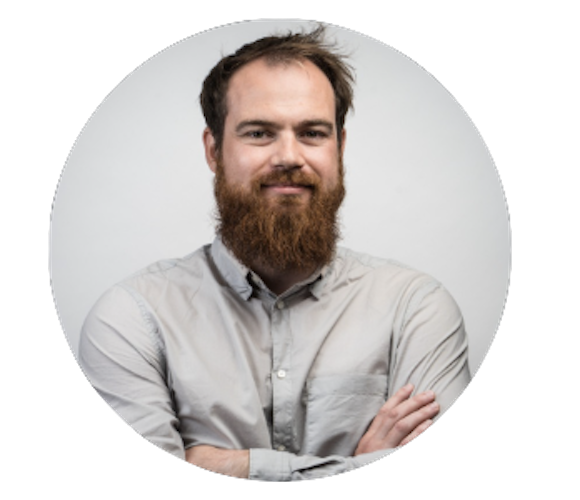
\includegraphics[width=\linewidth]{static/profilePicture.png}	%trimming relative to image size

%---------------------------------------------------------------------------------------
%	META SKILLS
%----------------------------------------------------------------------------------------
            \cvsection{SKILLS}

            \cvskill{Javascript} {7+ yrs} {1} \\[-2pt]

            \cvskill{NodeJs} {7+ yrs} {1} \\[-2pt]

            \cvskill{React} {4+ yrs} {0.70} \\[-2pt]

            \cvskill{Typescript} {4+ yrs} {0.70} \\[-2pt]

            \cvskill{Serverless} {3+ yrs} {0.5} \\[-2pt]

            \cvskill{GraphQl} {3+ yrs} {0.5} \\[-2pt]

            \cvskill{GIT} {7+ yrs} {1} \\[-2pt]

            \cvskill{BDD (Sql,NoSql)} {7+ yrs} {1} \\[-2pt]


            \vfill\null
            \cvsection{CONTACT}

            \icontext{MapMarker}{12}{Brest, Paris}{black}\\[6pt]
            \icontext{MobilePhone}{12}{+33 (0)6 88 03 29 37}{black}\\[6pt]
            \iconemail{Envelope}{12}{roland.paire@gmx.fr}{roland.paire@gmx.fr}{black}\\[6pt]
            \iconhref{Linkedin}{12}{roland-paire}{rhttps://www.linkedin.com/in/roland-paire/}{black}\\[6pt]

            \vfill\null
            \cvqrcode{0.7}

%---------------------------------------------------------------------------------------
%	EDUCATION
%----------------------------------------------------------------------------------------
            \newpage
            \cvsection{\'Etudes}

            \cvmetaevent
            {2012 - 2013}
            {Masters degree, Complementary skills in computer}
            {University Rennes 1}
            {Main thematic : Programming introduction (caml), Programming 1 and 2 (Java), Web conception (HTML, CSS, PHP, JavaScript, Ajax), Algorithm 1 and 2 (C++), XML, Language C, C++, Analyse (UML), System 1 and 2 (Assembly, Java), Data base (MySql), caor.}

            \cvmetaevent
            {2010 - 2012}
            {Masters degree, Modelisation of biological systems}
            {University de Rennes 1}
            {Main thematic : Programming (Python), Algorithm (Scilab), Population dynamics (R), Maths : statistic probabili- ties, Bayesian introduction, Sensibility analysis, SIR model, Epidemiology.}

            \cvmetaevent
            {2007 - 2010}
            {Degree, cellular biology and physiology}
            {University of Western Brittany}
            {Main thematic : Physiology, Genetics, Maths, Bioinformatics (Statistiques tests), Biochemistry, Molecular biology, Marine biology, Plant biology, Animal biology, Biotechnology, Population dynamics.}

            \vfill\null
            \cvqrcode{0.7}

        \end{leftcolumn}
        \begin{rightcolumn}
%---------------------------------------------------------------------------------------
%	TITLE  HEADER
%----------------------------------------------------------------------------------------
            \fcolorbox{white}{darkcol}{\begin{minipage}[c][3.5cm][c]{1\mpwidth}
                                           \begin {center}
                                               \HUGE{ \textbf{ \textcolor{white}{ \uppercase{ Roland PAIRE } } } } \\[-18pt]
                                               \textcolor{white}{ \rule{0.1\textwidth}{1.25pt} } \\[4pt]
                                               \large{ \textcolor{white} {Senior Software Developer Fullstack - Freelance} }
                                           \end {center}
            \end{minipage}} \\[12pt]
            \vspace{0pt}

%---------------------------------------------------------------------------------------
%	PROFILE
%----------------------------------------------------------------------------------------
%            \vfill\null
%            \cvsection{PROFILE}
%
%            \cvtext{IT Consultant with strong theoretical skills and a passion for OpenSource sofware.\\
%
%            DevOps Engineer, specialized both in automation and in custom application development, experienced with large projects and heterogeneous infrastructures. The link between development and operations, comfortable in both.\\
%
%            Customer-oriented and structured method of working, focused on quality and maintainability. Highly motivated to work in a team, both comfortable in big companies as in small teams.\\
%
%            }

%---------------------------------------------------------------------------------------
%	WORK EXPERIENCE
%----------------------------------------------------------------------------------------
%            \vfill\null
            \cvsection{WORK EXPERIENCE}

            \cvevent
            {Nov 21 - Jan 23}
            {Senior software developer}
            {Heyday by Hootsuite, Montreal, Canada}
            {Development of an application to improve the web presence of businesses on different channels (Messenger, Twitter, Instagram, WhatsApp) via a dashboard to centralize all the channels and a chatbot on the web site.}
            {\cvlist{
                \item Architecture design to move from a monolith to micro-services and a SaaS-type API
                \item Integration of Hootsuite and Heyday software
                \item Training new developers
                \item Maintenance of existing infrastructure
                \item Design and implementation of authentication and authorization services (SSO)
            }}
            {\cvlist {
                \item NestJs, NodeJs, Micro-service, serverless, SaaS, Gitlab, Typescript, AWS, DynamoDb, Lambda, SQS
                \item OpenAPI, Agile, project monitoring and planning, technical feasibility and technical debt study
            }}

%            \vfill\null
            \cvevent
            {Avr 20 - Nov 21}
            {Backend Developer, freelance}
            {Heyday, Montreal, Canada}
            {Development of a chatbot to improve the work of support teams and improve sales on e-commerce website.}
            {\cvlist{
                \item Integration of third-party APIs for the chatbot {\small(Prestashop, shopify, salesForce, ...)}
                \item Integration of communication channels {\small(Whatsapp, instagram, ...)}
                \item Maintenance and development of new features for the chatbot
                \item Upskilling of new developers on the product
                \item POC on new technology
            }}
            {\cvlist {
                \item NodeJs, Typescript, NoSql, cloudformation, AWS, Dynamodb, lambda, IAM, GitLab
                \item Agile, autonomy, functional and technical analysis, TDD, functional writing
            }}

%            \vfill\null
            \cvevent
            {Nov 16 - D\'ec 20}
            {Co-founder et CTO}
            {Hotel Skipper, Brest, France}
            {Development of a SaaS management control application for hotels.}
            {\cvlist{
                \item Study of the practices of hoteliers in the management of their operations
                \item Design of the web application and a software architecture
                \item Choice of technologies adapted to the project to limit the technical debt
                \item Creation of a POC, and deployment of marketable versions
                \item Management of a team of 5 developers
                \item Design of micro-services architecture
                \item Setting up continuous deployment with automatic tests  (TDD)
            }}
            {\cvlist {
                \item AWS, NodeJs, NestJs, React, Typescript, GraphQl, MongoDB, Github, Météor
                \item Agile, Architecture design, team management
            }}

            \cvevent
            {Mai 14 - Nov 16}
            {Business Intelligence Developer}
            {Sopra Steria group, Nantes, France}
            {Development and maintenance of BI applications for the client RTE.}
            {\cvlist{
                \item Realization of impact studies and quotes
                \item Sofwtare development based on customer needs
                \item Sofwtare maintenance
                \item Informatica and Shell trainer
                \item Lead Developer
                \item Implementation of test automation tools
            }}
            {\cvlist {
                \item ETL Informatica, Java, Javascript, Html/css, Shell, Oracle, SQL, Jenkins
                \item Creation and management of training
            }}

            \cvevent
            {Avr 13 - Sep 13}
            {Development Engineer Internship}
            {Thales Underwater Systems, Brest, France}
            {Artificial intelligence of an underwater drone.}
            {\cvlist{
                \item Development of an expert system in Prolog
                \item Implementation of an AI to find the best trajectory of the drone
                \item Setting up a web service in Java
            }}
            {\cvlist {
                \item Prolog, Java, PostgreSql
                \item Algorithm A*
            }}

% hotfixes to create fake-space to ensure the whole height is used
            \mbox{}
            \vfill
            \mbox{}
            \vfill
            \mbox{}
            \vfill
            \mbox{}
        \end{rightcolumn}
    \end{paracol}
\end{document}
